\documentclass[10pt]{article}
\usepackage[margin=0.78in]{geometry}
\usepackage{amsmath,amssymb,amsthm,mathtools}
\usepackage{graphicx}
\usepackage{xcolor}
\usepackage{microtype}
\usepackage[hidelinks]{hyperref}
\setlength{\parindent}{0pt}
\setlength{\parskip}{5pt}
\newtheorem{theorem}{Theorem}
\newtheorem{lemma}[theorem]{Lemma}
\newcommand{\K}{\mathbb K}
\newcommand{\Qp}{\mathbb Q_p}
\newcommand{\T}{\mathbb T}
\newcommand{\N}{\mathbb N}

\title{A Null-Diagonal Counterexample to Four\\Continuous Zauner Conjectures\\
\large Full negative answer for Conjectures 2.8, 2.9, 3.7, and 3.8 of arXiv:2209.12833}
\author{Automated proof attempt\\
\texttt{agent\_lane\_03} \quad model: GPT5.6}
\date{11 August 2026}

\begin{document}
\maketitle

\begin{center}
\fcolorbox{red!55!black}{red!4}{\parbox{0.92\linewidth}{
\textbf{Status: full counterexample, likely valid, pending human verification.}
All four conjectures are false as literally stated.  On any infinite compact
group with normalized Haar measure, the diagonal has product measure zero,
whereas the conjectures require it to equal a strictly positive quantity.}}
\end{center}

\section*{Source statements}

The source's Conjectures 2.8 and 2.9 (printed pp.~7--8) are respectively the
continuous non-Archimedean functional and Hilbert-space Zauner conjectures.
Conjectures 3.7 and 3.8 (printed pp.~14--15) are their \(p\)-adic analogues.
Every one is quantified over a given locally compact group \(G\) and every
dimension \(d\), and every one includes the exact equality
\begin{equation}\label{eq:source}
 |(\mu_G\times\mu_G)(\Delta)|
 =\text{(an off-diagonal correlation modulus)}
 =\frac{|\mu_G(G)|^2}{|d|},
 \qquad \Delta=\{(g,g):g\in G\}.
\end{equation}
The appended source excerpts reproduce the four statements and the decisive
equalities exactly.

\begin{theorem}[Simultaneous counterexample]\label{thm:counter}
Let \(G\) be any infinite compact group with normalized Haar probability
measure; in particular, take the circle group \(G=\T\).  Then none of
Conjectures 2.8, 2.9, 3.7, or 3.8 is true for \(G\).  Each fails already in
dimension \(d=1\).
\end{theorem}

\section*{Proof intuition}

The conjectures ask a continuously indexed family to be equiangular even on
the diagonal at the level of measure: they identify the measure of the
diagonal in \(G\times G\) with the nonzero correlation constant.  But Haar
measure on an infinite compact group has no atoms.  Consequently the diagonal
is a product-null set.  No choice of vectors, functionals, field, or frame
operator can repair the resulting equation \(0=1\) in dimension one.

\section*{Proof}

Let \(\mu\) be normalized Haar measure on an infinite compact group \(G\).
Every singleton has the same measure \(a=\mu(\{e\})\).  If \(a>0\), arbitrarily
large finite sets would have measure \(Na\), contradicting \(\mu(G)=1\).
Thus \(\mu(\{g\})=0\) for every \(g\in G\).  Tonelli's theorem now gives
\begin{equation}\label{eq:diag}
 (\mu\times\mu)(\Delta)
 =\int_G \mu\bigl(\{h:(g,h)\in\Delta\}\bigr)\,d\mu(g)
 =\int_G\mu(\{g\})\,d\mu(g)=0.
\end{equation}

Set \(d=1\).  Since \(\mu(G)=1\) and the absolute value of the multiplicative
unit is one, the right-hand side of \eqref{eq:source} is
\[
 \frac{|\mu(G)|^2}{|d|}=\frac{|1|^2}{|1|}=1.
\]
Equations \eqref{eq:source} and \eqref{eq:diag} would therefore require
\(0=1\).  This contradiction occurs before any of the vector, functional,
integrability, tightness, or diagonalizability conditions are used, so it
simultaneously refutes the functional and Hilbert-space versions.

For the non-Archimedean pair the hypothesis on the field is nonvacuous: for
example, \(\K=\mathbb R((t))\) with the \(t\)-adic absolute value satisfies the
source's equation (1), because the lowest-order coefficients in a finite sum
of squares of real Laurent series cannot cancel.  For the \(p\)-adic pair use
\(\Qp\), for any prime \(p\).  In either case \(|1|=1\), so the same
contradiction applies. \qed

\begin{theorem}[Finite-group obstruction]\label{thm:finite}
If a locally compact group \(G\) supports all the conditions in any one of the
four conjectural lists (for even one dimension), then \(G\) is finite.
\end{theorem}

\begin{proof}
In the functional formulations, choose a basis \((e_i)_{i=1}^d\) and its
coordinate functionals \((e_i^*)\).  Condition (i) makes each function
\(g\mapsto f_g(e_i)e_i^*(\tau_g)\) integrable, while self-normalization gives
\[
 1=f_g(\tau_g)=\sum_{i=1}^d f_g(e_i)e_i^*(\tau_g).
\]
Hence the constant function one is integrable and \(\mu_G(G)<\infty\).  The
same argument in the Hilbert formulations uses
\(1=\langle\tau_g,\tau_g\rangle\) and an orthonormal coordinate basis.  A
locally compact group has finite Haar measure exactly when it is compact.

The exact equality \eqref{eq:source} has a nonzero right-hand side, so
\((\mu_G\times\mu_G)(\Delta)>0\).  Haar invariance and Tonelli give
\[
 (\mu_G\times\mu_G)(\Delta)=\mu_G(G)\mu_G(\{e\}),
\]
and thus \(\mu_G(\{e\})>0\).  As above, positive singleton mass is incompatible
with infinitely many points in a compact neighborhood; consequently \(G\) is
discrete.  A compact discrete group is finite.
\end{proof}

\section*{Scope and literature boundary}

The theorem fully refutes the four universal conjectures.  It does not fully
classify Questions 2.6, 2.7, 3.5, and 3.6: those use a maximum of the diagonal
mass and the off-diagonal correlation, so a null diagonal need not contradict
their equality.  A natural repair of the conjectures would restrict \(G\) to
finite groups or remove the demand that the diagonal mass itself equal the
correlation constant.

No exact-ID duplicate was found in the run indexes.  Exact conjecture-name and
arXiv searches through 11 August 2026 returned the source and its companion
discrete papers, but no later correction or counterexample.  This is a bounded
novelty check, not an exhaustive priority claim.  The nearby run packet for
arXiv:2210.07062 concerns a discrete repeated-vector degeneracy; the present
measure obstruction is distinct and specific to the continuous statements.

The script \path{code/verify_diagonal_measure.py} checks that normalized finite
cyclic groups have diagonal product mass \(1/N\), tending to the exact
nonatomic value zero.  The proof itself is the measure identity
\eqref{eq:diag} and has no computational dependency.

\begin{thebibliography}{9}
\bibitem{source}
K. Mahesh Krishna, \emph{Continuous Non-Archimedean and p-adic Welch Bounds},
arXiv:2209.12833 (2022).  Included as \texttt{source\_paper.pdf}.
\end{thebibliography}

\clearpage
\section*{Exact source excerpt: non-Archimedean conjectures}
\begin{center}
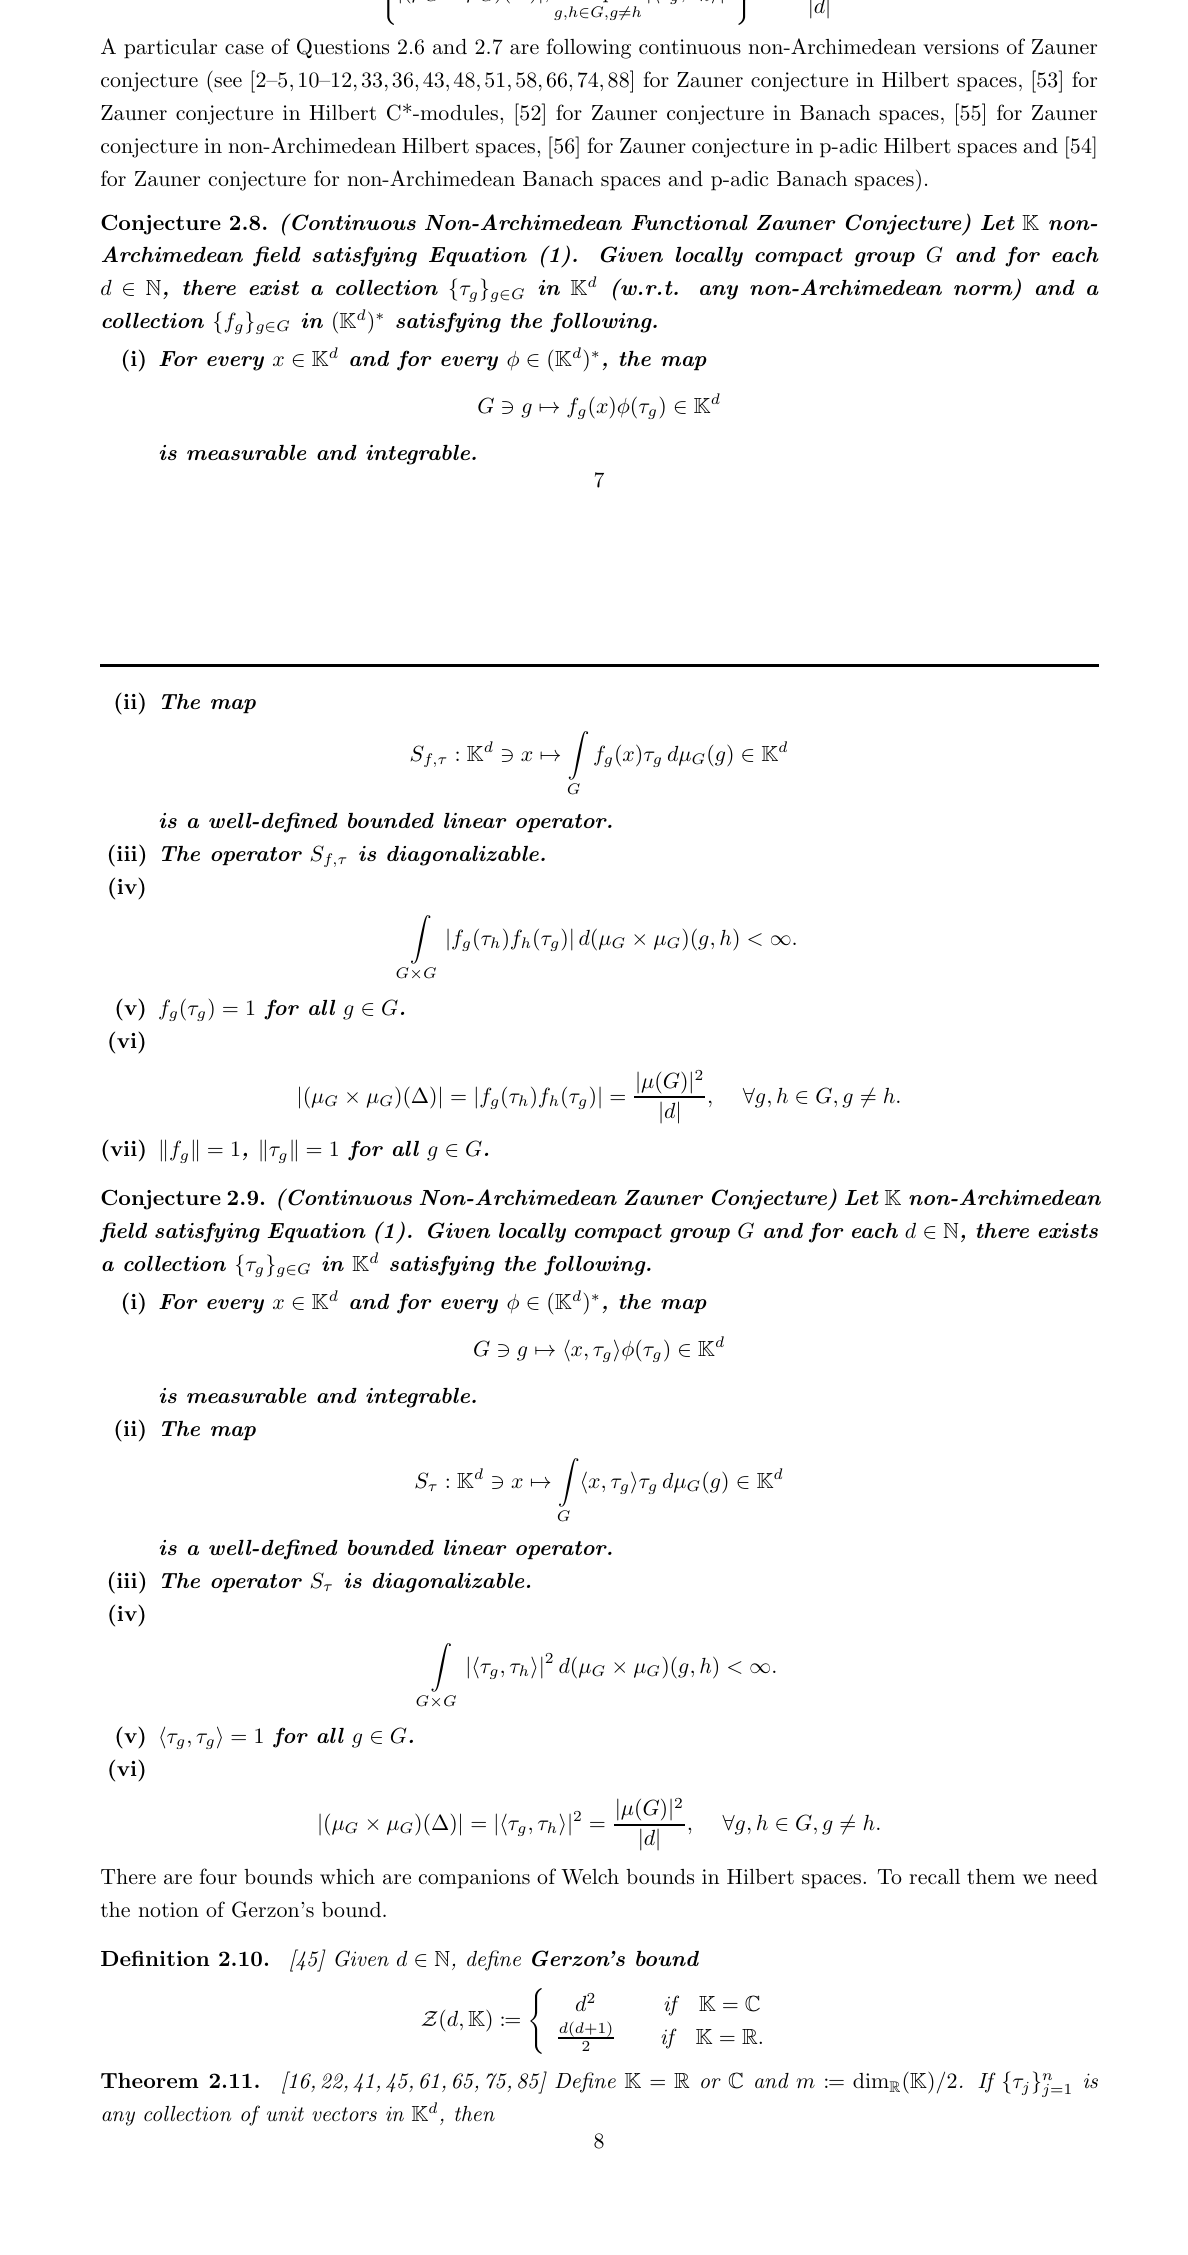
\includegraphics[height=0.74\textheight,keepaspectratio]{source_nonarch_crop.png}
\end{center}

\clearpage
\section*{Exact source excerpt: \(p\)-adic conjectures}
\begin{center}
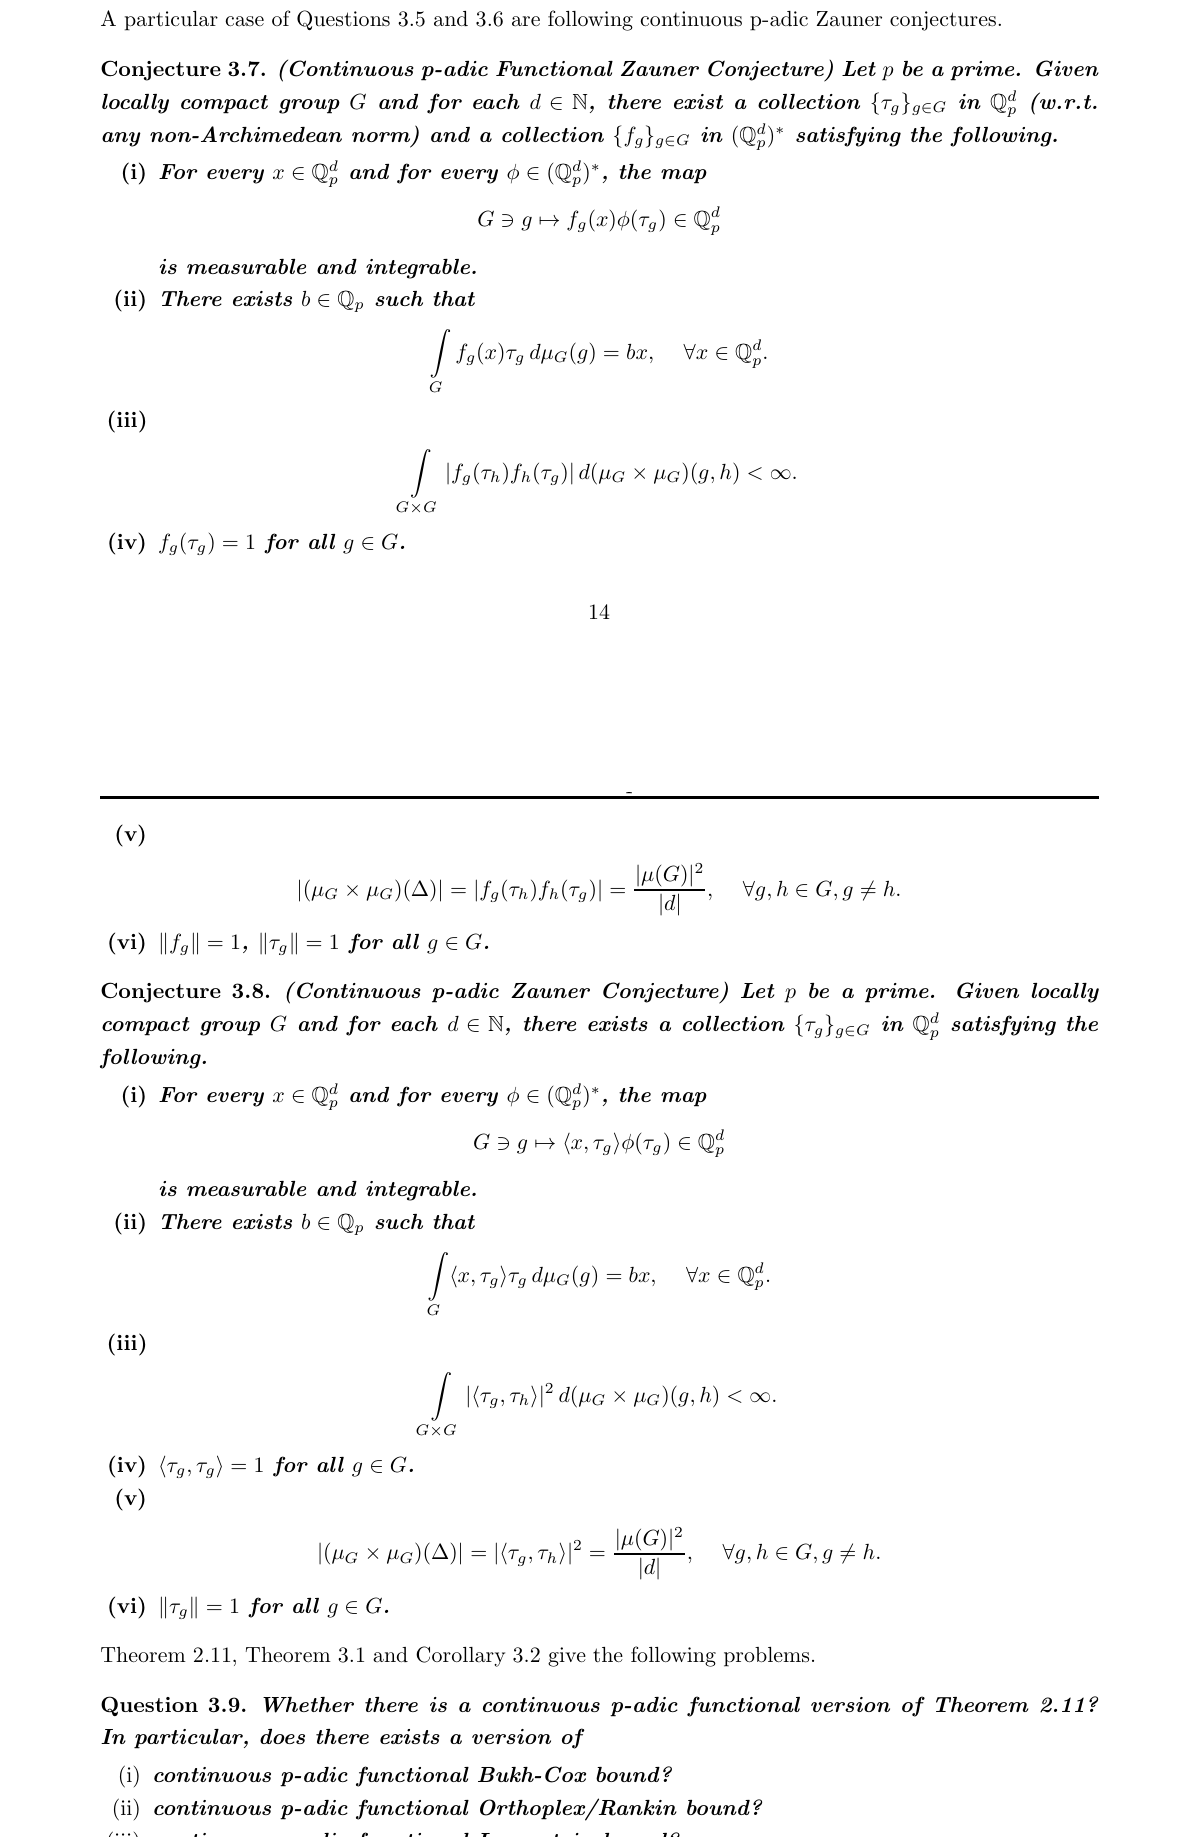
\includegraphics[height=0.74\textheight,keepaspectratio]{source_padic_crop.png}
\end{center}

\end{document}
